%-*- mode: latex; fill-column: 70 -*-
% ex: set sts=4 ts=4 sw=4 et tw=70:
%&pdflatex

\documentclass[letterpaper,landscape]{report}
\usepackage[landscape,margin=0.5cm]{geometry}
\usepackage{color}
\usepackage{flowfram}
\usepackage[colorlinks]{hyperref}

\usepackage{multicol}
\setlength{\columnseprule}{1pt} % for visible divider
\setlength{\columnsep}{1cm}

\usepackage{graphicx}
\graphicspath{
 {../}
}

\usepackage{enumitem}           % useful for control of listings
\usepackage[compact,raggedleft]{titlesec}
\usepackage{comment}

\newcommand{\epigraph}[3]{\textit{#1}\linebreak \vspace{-1.5em} \begin{flushright}\hspace{5em}\ --\ #2\linebreak\small{#3} \end{flushright}}

\pagestyle{empty}
\parindent=0pt

% Attempts to change bg color of *section headings
%\definecolor{secbgcol}{rgb}{0.9, 0.85, 0.85}
%\titleformat{\section}
%{\color{red}\normalfont\Large\bfseries}{\thesection}{1em}{}
%\titleformat{\subsection}
%{\color{red}\normalfont\large\bfseries}{\begin{flushright}\hfill\thesubsection
%  \end{flushright}}{1em}{}
%

\begin{document}

%%
%% DEBIAN
%%
\begin{multicols}{3}    % 3 columns

\begin{center}
\noindent
\includegraphics[width=0.5\columnwidth]{openlogo}
%
\includegraphics[width=0.5\columnwidth]{openlogo-vsop}

\url{http://www.debian.org}
%\section*{Debian GNU/Linux}

\section*{The Universal Operating System}
\hrule
\end{center}
\vspace{-1em}

\section*{Debian project}
was founded by Ian Murdock in August 1993 with the goal
to create an easy to install and maintain non-commercial GNU/Linux
distribution that would be able to effectively compete in the
commercial market.  Since then Debian established itself as an
independent and unique project driven by more than 3,000 of
enthusiastic Debian developers and contributors all around the globe.
Principles of \emph{do-ocracy} and democracy backed up by evolving open
standards allowed Debian to deliver the comprehensive operating system largest not
only in its coverage of integrated software, but also in the
number of the supported hardware architectures.
% Current installer of Debian has been translated more that to 60 languages.
% (12 ???  officially supported architectures).
% Well appreciated
Acknowledged quality and openness of Debian made it the choice for
more than 120 derivative GNU/Linux distributions, such as Ubuntu and
Mint.

\subsection*{Debian is}
\begin{description}[nolistsep,leftmargin=0.8em]
\item[V\textnormal{ersatile}]\hfill\url{http://packages.debian.org}\\
  Over 15,000 software products maintained to provide
  a stable system for any field of application
\item[S\textnormal{ecure}]\hfill\url{http://www.debian.org/security}\\
  Security updates guarantee virus-free safe operation
%\item[S]table
% \item[S\textnormal{imple}]\blank\\
%   Single command is enough to install or upgrade single
%   software or the entire system at once
\item[O\textnormal{pen}]\hfill\url{http://www.debian.org/social_contract}\\
  All software is free and open-source (FOSS).\\
  Debian project decisions are voted for in public
\item[P\textnormal{opular}]\hfill\url{http://www.debian.org/users}\\
  Used by governments, companies, education institutions
\end{description}

\begin{comment}
Original: Very Special Old Pale

Could also stand for
Very (Special|Stable) Operating Platform
\end{comment}

%\section*{Understand Debian}
\columnbreak
\subsection*{Debian suites}

% Debian distribution comes in 3 major flavors

\begin{description}[nolistsep,leftmargin=1pc,topsep=1em]

%\item[Unstable] \emph{Constantly changing distribution}\\
\item[Development]\hfill\emph{Unstable} (always \emph{sid})\\
  Never \emph{released}, constantly evolving platform to integrate new
  versions of software in Debian.\\
  %entry point for the software to appear in Debian.\\
  Despite its name, \emph{Unstable} is a good platform for those
  requiring the most recent versions of software

%\item[Testing] \emph{Constantly changing future release candidate}\\
\item[``Always-ready-to-release'']  \emph{Testing} (now \emph{squeeze})\\
%  What to become a next \emph{Stable} release candidate.\\
  Software versions known to be secure and of good quality.
%  Software migrated from \emph{Unstable} which is known to be of good
%  quality.  Immediate updates are provided only
%  to assure secure and robust performance. \\
  \emph{Testing} provides a good balance between stability and recency
  of software

%\item[Stable] \emph{Official release}\\
\item[Official release]\hfill\emph{Stable} (now \emph{lenny})\\
  % Software verified to be well tested and secure,
  % Very stable (hence the name) and secure
  % but might be lacking the most recent versions.\\% of the software.\\
  % of not the most recent versions. \\
  \emph{Stable} is released ``when it is ready'', \emph{i.e.} when
  \emph{Testing} is assured to be robust. %, on average bi-yearly.
  Complementary updates keep the
  system secure. \\
  \emph{Stable} is the choice where stability and security are of
  primary importance.
\end{description}

\begin{comment}
\subsection*{It has names}

The code names of Debian releases are names of characters from the Toy
Story animation, e.g. sid, squeeze, lenny.  \emph{Unstable}
flavor always called \emph{sid}, while a new name chosen for every
upcoming release and assigned to \emph{Testing} to become a code name
of the release when it becomes \emph{Stable}.\\  At the moment
\emph{squeeze} is \emph{Testing}, and \emph{lenny} is \emph{Stable}.
As soon as \emph{squeeze} gets released, \emph{Testing} will be given
a new name -- \emph{wheezy}.
\end{comment}

\subsection*{Debian components}

% Debian distribution comes in 3 major flavors
%Debian Free Software Guidelines (DFSG)\\
%\url{http://www.debian.org/social_contract}

\begin{description}[nolistsep,leftmargin=1pc,topsep=1em]
\item[Free as in freedom]\hfill\emph{main}\\
  % This is the actual Debian with full support.\\
  All software in \emph{main} is distributed under FOSS licenses
  compliant with Debian Free Software Guidelines (DFSG) to assure
  complete freedom to use, modify, and (re-)distribute
\item[Not free \emph{en bloc}]\hfill\emph{contrib}\\
  FOSS depending on \emph{non-free} 3rd party software
%  Software which, despite being free itself, depends on
%  \emph{non-free} 3rd party software, rendering it useless without
\item[Somewhat free]\hfill\emph{non-free}\\
  Software under restrictive licenses
 % removing some freedoms
 % (\emph{e.g.} non-commercial use only), but which is allowed to be
 % used for free and re-distributed (\emph{e.g. NVidia drivers})
\end{description}


\subsection*{Debian is driven by enthusiastic experts}
% could be simply 'Debian People' or 'Debian Community'

Debian is the only major Linux distribution developed
cooperatively solely by individuals through the Internet, in the
same spirit as Linux and other FOSS.\\
Debian developers, teams and the community contribute to the
project not by writing new applications (in most cases), but by
\begin{itemize}[nolistsep,topsep=0em,leftmargin=1pc]
\item integrating existing software into Debian
\item fixing and communicating bug reports to upstream developers
\item assuring overall quality of the distribution
\item improving documentation and internationalization
\item providing user support
\end{itemize}

Packaged software in Debian have individual maintainers which are
often also the users of that software, so they are interested in its
reliable operation.  Individual maintainers often join the teams, such
as Debian-Science or Debian-Med, based on the common field of
interest.

%\columnbreak
\subsection*{HOWTO get Debian}

%\subsubsection*{Stable}
\begin{description}[nolistsep,leftmargin=1pc,style=nextline]
\item[Install on a hard-drive] \url{http://get.debian.net/}
\item[Boot from CD/USB] \url{http://get.debian.net/live/}
\item[Run in a Virtual Machine] \url{http://neuro.debian.net/vm.html}
\item[More options (e.g. buy pre-installed)] \url{http://debian.org/distrib}
\item[Testing/Unstable version] \url{http://www.debian.org/devel/debian-installer}
\end{description}

% \subsection*{Get \emph{Testing/Unstable} Debian}
%
% Install on a hard-drive or in a Virtual Machine\\
% \url{http://www.debian.org/devel/debian-installer}
%

\subsection*{HOWTO install software X}

\begin{description}[nolistsep,leftmargin=1pc,style=nextline]

\item[GUI (Synaptic Package Manager)]
%  \emph{Synaptic Package Manager}
  Select X and click ``Apply''\\
  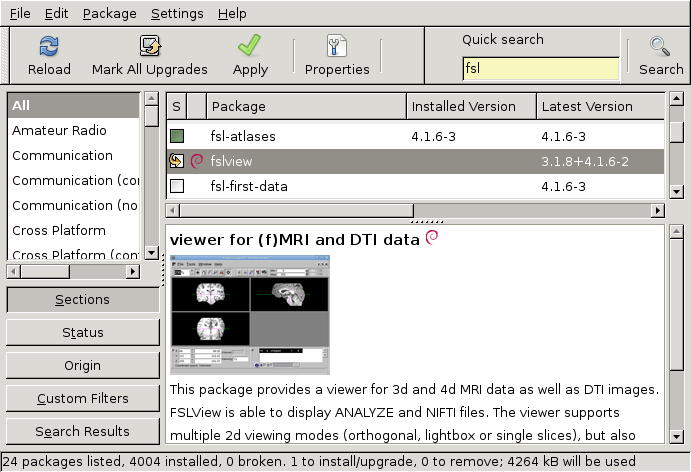
\includegraphics[width=0.95\columnwidth]{shots/synaptic-fslview}
\item[Command line]
  apt-get install X
\end{description}



\subsection*{HOWTO upgrade the entire system}

\begin{description}[nolistsep,leftmargin=1pc,style=nextline]
\item[GUI (Synaptic Package Manager)]
  Click ``Mark All Upgrades'', ``Apply''
\item[Command line]
  apt-get update; apt-get dist-upgrade
\end{description}

\subsection*{HOWTO get support}

\url{http://www.debian.org/support}

\begin{description}[nolistsep,leftmargin=1pc,style=nextline]
%\item[GUI]
%  Use \emph{Synaptic Package Manager}
\item[Software bug]
  reportbug X
\item[Community support]
  %\begin{description}[nolistsep,leftmargin=1pc]
  %\item[Mailing lists] 
  \url{http://www.debian.org/MailingLists}\\
  \url{http://forums.debian.net}\\
  \url{http://ask.debian.net}
  %\end{description}
\item[Commercial support]
  \url{http://www.debian.org/consultants}
\end{description}

\begin{comment}
\section*{Reasons to choose Debian}
\paragraph{It is maintained by its users}

If something needs to be fixed or improved, we just do it.

\paragraph{Unparalleled support}

Mail sent to the mailing lists often gets answers within 15 minutes (or less),
for free, and by the people who developed it. Compare that to typical phone
support: hours spent on the phone, for money, only to get someone who doesn't
know the system well enough to even understand your question.

\paragraph{You wouldn't be alone in your choice}

A wide range of organizations and individuals use Debian. See our Who's Using
Debian? page for a description of some high-profile sites which use Debian, and
have chosen to submit a short description of how they use Debian and why.

\paragraph{The best packaging system in the world.}

Tired of old files from software three versions old cluttering your system? Or
installing a piece of software only to find it causes your system to crash
because of software conflicts? Dpkg, Debian's endured packaging system, takes
care of these issues for you.

\paragraph{Easy installation}

If you have heard that GNU/Linux is difficult to install, then you haven't
tried Debian lately. We are constantly improving the installation process. You
can do the installation directly from CD, DOS, floppies or even over the
network.

\paragraph{Incredible amounts of software}

Debian comes with over 25000 different pieces of software. Every bit of it is
free. If you have proprietary software that runs under GNU/Linux, you can still
use it - in fact, there may even be an installer in Debian that will
automatically install and set up everything for you.

\paragraph{Packages well integrated}

Debian surpasses all other distributions in how well its packages are
integrated. Since all software is packaged by a coherent group, not only can
all packages be found at a single site, but you can be assured that we have
already worked out all issues regarding complicated dependencies. While we feel
that the deb format has some advantages over the rpm format, it is the
integration between the packages that makes a Debian system more robust.

\paragraph{Source code}

If you are a software developer, you will appreciate the fact that there are
hundreds of development tools and languages, plus millions of lines of source
code in the base system. All of the software in the main distribution meets the
criteria of the Debian Free Software Guidelines (DFSG). This means that you can
freely use this code to study from, or to incorporate into new free software
projects. There are also plenty of tools and code suitable for use in
proprietary projects.

\paragraph{Easy upgrades}

Due to our packaging system, upgrading to a new version of Debian is a snap.
Just run apt-get update ; apt-get dist-upgrade (or aptitude update; aptitude
dist-upgrade in newer releases) and you can upgrade from a CD in a matter of
minutes or point apt at one of the over 300 Debian mirrors and upgrade over the
net.

\rotatebox{90}{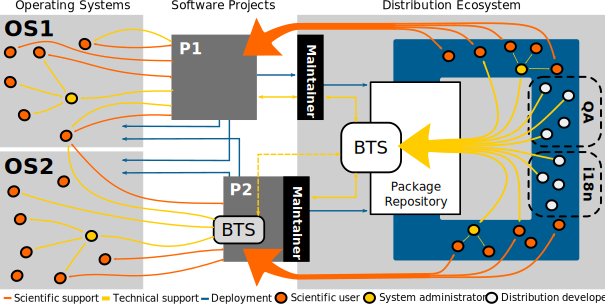
\includegraphics[height=.9\columnwidth]{distro-dev}}
\rotatebox{90}{Description}

\paragraph{Multiple architectures and kernels}

Currently Debian supports an impressive number of CPU architectures: alpha,
amd64, armel, hppa, i386, ia64, mips, mipsel, powerpc, s390, and sparc. It also
runs on GNU Hurd and FreeBSD kernels besides Linux, and with the debootstrap
utility you will be hard-pressed to find a device that can't run Debian.

\paragraph{Bug tracking system}

Debian's bug tracking system is publicly available. We don't try to hide the
fact that software doesn't always work the way users want. Users are encouraged
to submit bug reports and are notified when and why the bug was closed. This
system allows Debian to respond to problems quickly and honestly.


\section*{Acknowledgements}
\end{comment}

\end{multicols}


\pagebreak
%%
%% NeuroDEBIAN
%%
\begin{multicols}{3}    % 3 columns

\begin{center}
\noindent
\vspace{-3em}
\includegraphics[width=\columnwidth]{logo_tuned/label}

\url{http://neuro.debian.net}
%\section*{NeuroDebian Project:}
\section*{The Ultimate Research Platform}
\hrule

\end{center}

\section*{NeuroDebian}

is a Debian project aiming to provide Neuroscience community with a
stable and versatile research platform -- the Debian OS.  NeuroDebian
(formerly known as Experimental Psychology, ExpPsy) was initiated in
2006 to provide packaging of PyEPL and FSL software so they could
become an integral part of Debian, thus seamlessly available to users
of Debian or any derived distribution.  Since 2006 software coverage
of NeuroDebian increased more than ten-fold.  NeuroDebian repository
\url{http://neuro.debian.net} makes recent versions of the software
available not only for the \emph{Development} but also for previous
releases of Debian and Ubuntu.  The tandem of a stable generic
operating system, Debian, together with new versions of research
software from NeuroDebian repository compose the ultimate research
platform -- stable versatile environment with recent neuroscientific
methodologies just 1-click away.  Such stability, ease of software
installation and system maintenance and constantly growing coverage of
software solutions made NeuroDebian project popular among
neuroscientists and scientific software developers.


\subsection*{NeuroDebian is NOT}

a yet another Debian GNU/Linux derivative distribution.  All work done
within NeuroDebian project targets software inclusion in the official
Debian distribution.


\subsection*{Advantages from Debian integration}

\begin{itemize}[nolistsep,leftmargin=1pc]

% rephrase to outline the benefit, not burden
\item Debian standards and policies guaranty quality and robustness

\item Debian centralized bug tracking system provides a unified
  single-point of entry for bug reporting and troubleshooting for any
  software in Debian

\item Debian makes software available within world-wide distribution
  network, thus offloading bandwidth demands

\item Other Debian enthusiasts take care about large-scale aspects of
  deployment, quality assurance, porting and integration at the level
  of the entire distribution:

\begin{description}[nolistsep,leftmargin=1pc]
\item[Porting] Software sources get built for 11 hardware
  architectures and 3 kernels (Linux, HURD, kFreeBSD). Ports teams
  maintain build infrastructure and help making the code
  platform-agnostic.
\item[QA] Whole-archive rebuilds assure robustness of packaging and
  warn about upcoming problems (core libraries upgrades) beforehand.
\item[Internationalization (I18n)] I18n teams contribute by localizing
  software for more than 50 languages
\end{description}

\item Neuroscience software becomes 1st-class citizen within Debian
  project, which guarantees its availability, longevity, smooth
  installation and upgrades

\item Participation in the Debian community helps to assure Debian's
  aptness for the neuroscientific software demands

\end{itemize}


\subsection*{NeuroDebian coverage}
\begin{flushright}
\vspace{-0.5em}
\url{http://neuro.debian.net/pkgs.html}
\vspace{-1em}
\end{flushright}
\begin{description}[nolistsep,leftmargin=1pc,topsep=0em]
\item[Electrophysiology] BioSig, Sigviewer, Brian, \ldots
\item[Machine Learning] PyMVPA, scikits.learn, \ldots
\item[Medical Imaging] AFNI, Caret, FSL, Mricron, NiPy, Voxbo, \ldots
\item[Psychophysics] PsychoPy, PyEPL
\end{description}



%\columnbreak

\subsection*{HOWTO get NeuroDebian}
\begin{description}[nolistsep,leftmargin=1pc]
\item[Debian/Ubuntu]\url{neuro.debian.net} repository
\item[Others] NeuroDebian Virtual Machine
% Here place a left-top corner of OSX with seamless mode
\end{description}
\begin{comment}
\subsection*{Developers oriented information}

%\columnbreak

\subsection*{Who is using NeuroDebian}

\noindent
%\includegraphics[width=\columnwidth]{usage_worldmap}

buga dugabuga dugabuga dugabuga dugabuga dugabuga dugabuga dugabuga dugabuga dugabuga dugabuga dugabuga dugabuga dugabuga dugabuga dugabuga dugabuga dugabuga dugabuga dugabuga dugabuga duga
\end{comment}

\def\blank{\hspace{0em}\vspace{-1em}}
\columnbreak
\subsection*{Work-in-progress}

\begin{description}[nolistsep,leftmargin=1pc,topsep=1em,style=nextline]

\item[Expanded coverage]\blank
  \begin{description}[nolistsep,leftmargin=1pc,topsep=0em,style=nextline]
  \item[Electrophysiology] BioSig, Brian, NEURON, \ldots
  \item[Matlab/Octave toolboxes] SPM, EEGLAB, \ldots
  \end{description}
\vspace{0.5em}
\epigraph{Having FreeSurfer integrated into the Debian operating system by the NeuroDebian team would have enormous benefits for us, and for the thousands of users of FreeSurfer across the world.}{Prof. Bruce Fischl}{Director, Computational Core at Martinos Center at Massachusetts General Hospital, Charlestown, Massachusetts, USA}
\item[Improved quality assurance]
  Extended integration and regression testing
\item[Available snapshotting service]
  % Entire NeuroDebian repository for any given past moment
  All versions of packages readily available
\item[Data as the 1st class citizen]
  \url{http://neuro.debian.net/datasets.html}
\item[Universal availability]\blank
  % \begin{itemize}[nolistsep,leftmargin=1pc,topsep=0em]
  % \item Virtual Appliance enhancements
  %\item
  Cloud computing
  %\end{itemize}

\end{description}


\subsection*{Testimonials}
\begin{flushright}
\vspace{-0.5em}
\url{http://neuro.debian.net/testimonials.html}
\vspace{-1em}
\end{flushright}


\epigraph{The approach taken with NeuroDebian is plainly the most appropriate
approach to software distribution for the dominant platform in brain
image analysis, and I have great confidence that this project will be
a major asset to the neuroscience community in facilitating the
distribution of stable software, improving the reliability and
replicability of analyses, and in helping to improve software
development practices.}{Prof. Daniel Y. Kimberg}{Director, Data
Processing Facility, Center for Functional Neuroimaging, University of
Pennsylvania, Philadelphia, USA}

\subsection*{Acknowledgements}

We are grateful to all Debian developers and contributors for the
development of Debian OS, and to Prof. James V. Haxby (PBS Department,
Dartmouth College) for his continued support and endless supply of
Italian espresso (\url{http://neuro.debian.net/coffeeart.html}).

%\columnbreak
\end{multicols}



\end{document}


%%% Local Variables:
%%% mode: latex
%%% TeX-master: t
%%% TeX-PDF-mode: t
%%% whizzy-viewers: (("-pdf" "okular") ("-dvi" "xdvi") ("-ps" "gv"))
%%% End:
